\chapter{Medical Fundamentals}
 An important prerequisite to the work addressed in this thesis is comprehending the physiology of the human heart and the cardiovascular system. Therefore, the theoretical foundations of these topics will be introduced in the following chapter.

\section{Cardiovascular System}
The fundamental task of the cardiovascular system is to supply all organs with blood through circulation. The human cardiovascular system is divided into two components, the systemic circulation and the pulmonary circulation. The systemic circulation is supplying blood flow to all tissues and organs apart from the lungs. \figurename~ \ref{fig:circulation} represents the blood distribution over the circulatory system.  \cite{GH20}
\begin{figure}[ht]
  \centering
  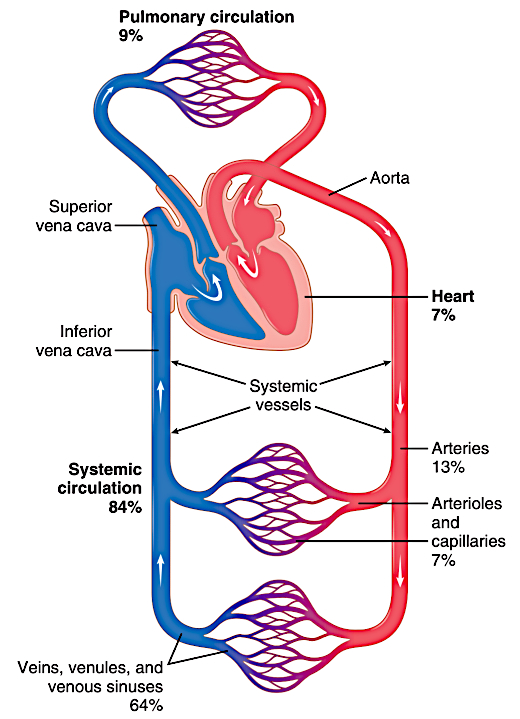
\includegraphics[width=0.4\textwidth, height=0.6\textwidth]{images/chapt_2/circulation.jpg}
  \caption[Blood distribution in the ciculatory system \cite{GH20}]{Blood distribution in the circulatory system \cite{GH20}. Red highlighting representing oxygenated, blue highlighting depicting deoxygenated blood flow.}
  \label{fig:circulation}
\end{figure}
 \\The center of the cardiovascular system is the heart. The heart itself consists of two mechanical pumps, which are functionally connected in series but are united in one organ. It is separated into two sides, which themselves are divided into an atrium and a ventricle each. The atria act as weak primer pumps required to provide blood flow to the ventricles. \cite{HKS4} Both the atria and the ventricles are surrounded by the myocardium, which serves as the working muscle of the heart. Through contraction of the myocardium, blood is pumped into the circulatory system. \cite{HKS7} The left ventricle is pumping oxygenated blood through the aorta into the systemic circulation. There, oxygen stored in the blood is delivered to the organs. The blood, now low in oxygen, is then led into the right atrium through the inferior and superior vena cava. From the right atrium, the deoxygenated blood then enters the right ventricle. Afterwards, it is directed into the pulmonary circulation via the pulmonary artery. When the blood is oxygenated in the lungs, it is returned to the left atrium through the pulmonary vein. \cite{HKS4} In addition to the atria and the ventricles, each side of the heart has an atrioventricular (A-V) valve, as well as a semilunar (SL) valve. The A-V valve of the left heart is called the mitral valve, the one of the right heart is referred to as the tricuspid valve. The aortic valve and pulmonary valve are the SL valves of the left and right heart, respectively. The valves determine the direction of blood flow and thus prevent backflow. \cite{HKS7} A graphic overview of the anatomy and the course of blood flow through the heart is provided by \figurename~\ref{fig:heart_anat}.
 \begin{figure}[!ht]
   \centering
   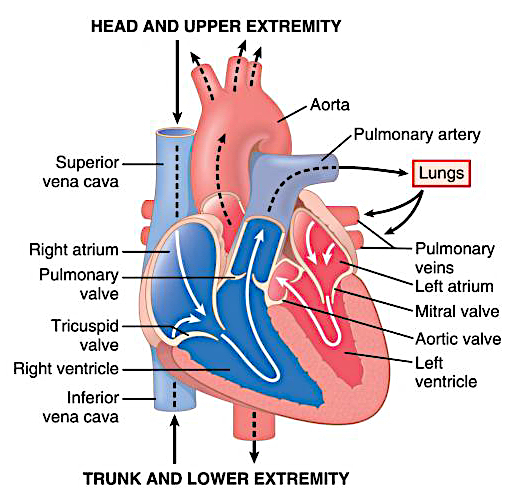
\includegraphics[width=0.55\textwidth]{images/chapt_2/heart_1.jpg}
   \caption[Anatomy of the human heart \cite{GH20}]{Anatomy of the human heart \cite{GH20}. Red highlighting representing oxygenated, blue highlighting depicting deoxygenated blood flow.}
   \label{fig:heart_anat}
 \end{figure}
\\ The amount of blood pumped through each side of the heart,  called cardiac output (CO), is equal at all times. It is determined by multiplying the heart rate (HR) by the stroke volume (SV). For an average adult at rest with a heart rate of approximately $70\, min^{-1}$ and a stroke volume of $70 \, ml$, this leads to
 \begin{equation}
   CO = HR \times SV = 70\, min^{-1} \times 70 \,ml = 5 \,\frac{l}{min}.
  \label{eq:CO}
 \end{equation}
In case of maximum physical load, given at a stroke volume of $110\,ml$ and a heart rate of $190 \, min^{-1}$,  the cardiac output can increase to up to $20\,\frac{l}{min}$. \cite{HKS4}
\\The cardiac cycle comprises all events that occur during the time-span of one heartbeat. The cycle is triggered by an electrochemical action potential originating from the sinus node. The cycle is divided into four phases. \figurename~ \ref{fig:cardiac_cycle} illustrates these action phases and events of the cardiac cycle for the left ventricle.
\begin{figure}[ht]
  \centering
  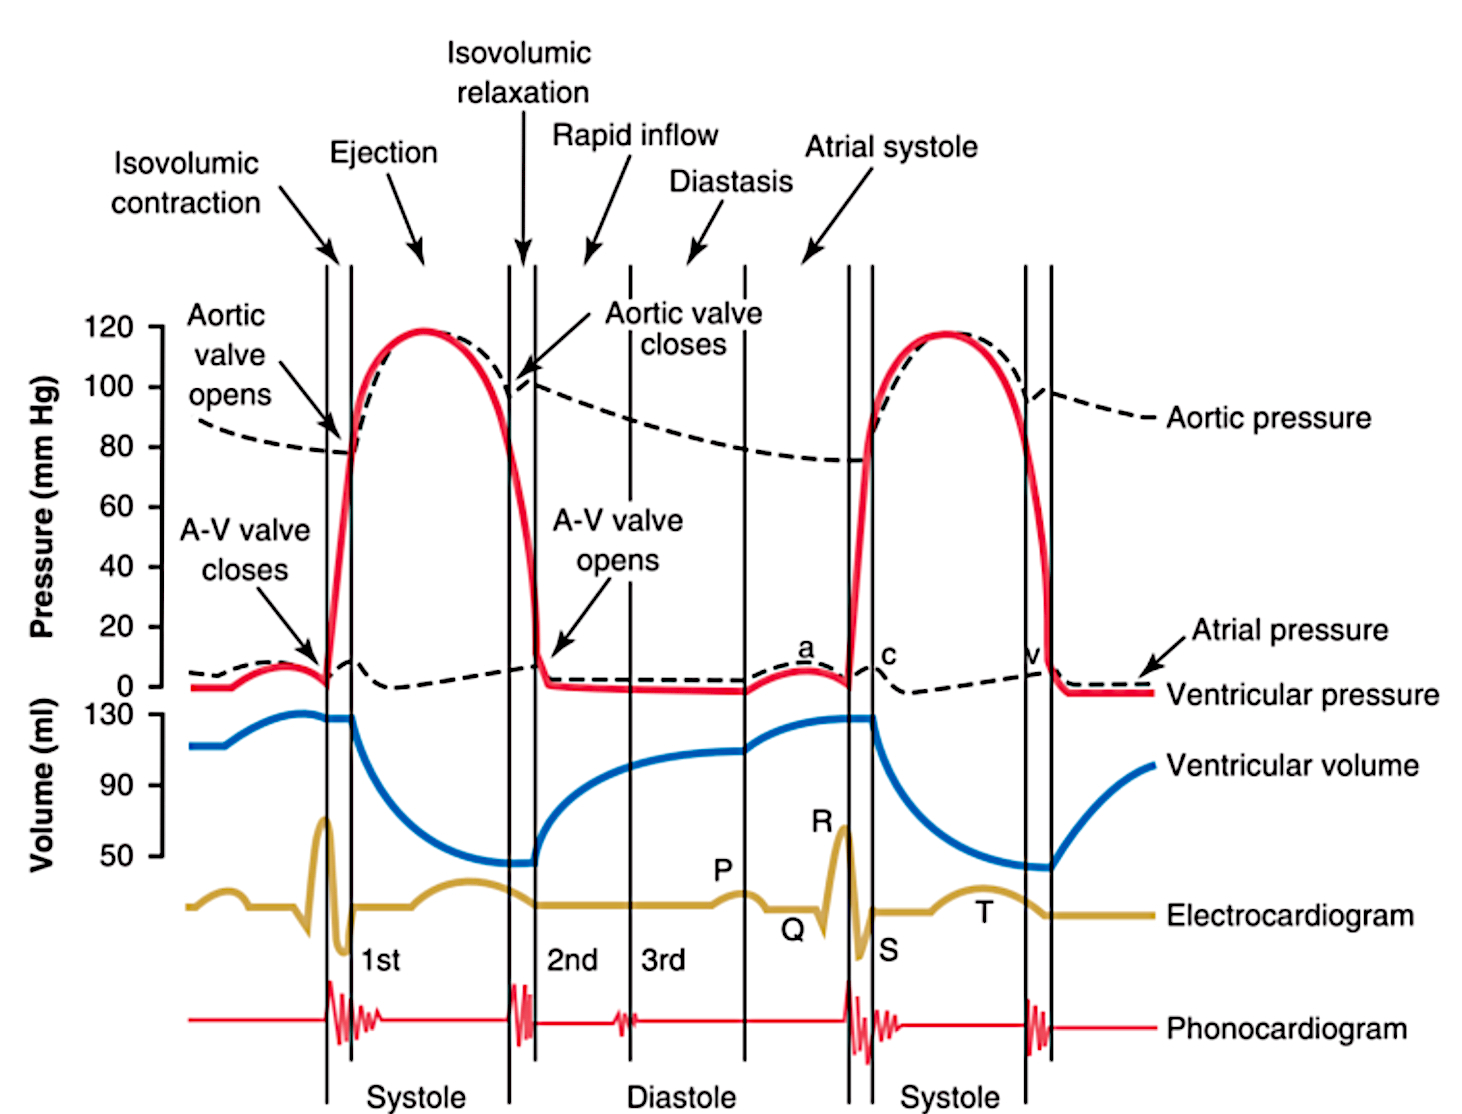
\includegraphics[width=0.8\textwidth]{images/chapt_2/cardiac_cycle.jpg}
  \caption[Action phases of left ventricular cardiac cycle \cite{GH20}]{Action phases of the cardiac cycle based on the example of the left ventricle \cite{GH20}.}
  \label{fig:cardiac_cycle}
\end{figure}
\\During the period of isovolumic contraction, the ventricular pressure increases. For the left ventricle, the pressure increases from about $4-6 \, mmHg$ to $80 \, mmHg$, whilst the pressure values for the right ventricle are much lower. This increase is occuring as a direct result of the ventricular contraction. The A-V valves, as well as the SL valves, are closed during this process, leading to a constant blood volume in the ventricles. As soon as the ventricular pressure exceeds the arterial pressure, the pulmonary and aortic valves open and blood can flow into the aorta and the pulmonary artery. This phase is called ejection phase, as the blood is ejected into the circulatory system. The period of isovolumic contraction combined with the ejection phase comprises the ventricular systole. \cite{HKS4} During the systole, the blood volume in the ventricle decreases by $55-60 \, \%$, resulting in an end-systolic volume (ESV) of about $40-50 \, ml$ \cite{GH20}. Due to the contraction of the myocardium, the ventricular pressure keeps increasing for a while before decreasing again as relaxation of the myocardium sets in. As soon as the outflow of blood ends, the semilunar valves close, initiating the period of isovolumic relaxation. During this period, pressure in the ventricles is decreasing while blood volume remains constant. When the pressure in the atrium exceeds the ventricular pressure, the A-V valves open. This leads to blood flowing into the ventricles until pressure levels in the atria and ventricles are equalized. \cite{HKS4} This phase is referred to as period of rapid filling of the ventricles. This period, in combination with the isovolumic relaxation, forms the diastole. The end-diastolic volume (EDV) amounts to about $110-120 \, ml$. \cite{GH20} While at rest, the diastole lasts about twice as long as the systole. Above a heart rate of $150 \, min^{-1}$ however, the two phases are about equal \cite{HKS4}.
\\The pumping mechanism of the left ventricle can be illustrated using a pressure-volume diagram (P-V diagram). Construction of the P-V diagram first requires discussing the relationship between the left ventricular volume and the ventricular pressure during diastole and systole, as displayed in \figurename~\ref{fig:pv_1}.
\begin{figure}[ht]
  \centering
  \subfloat[]
  {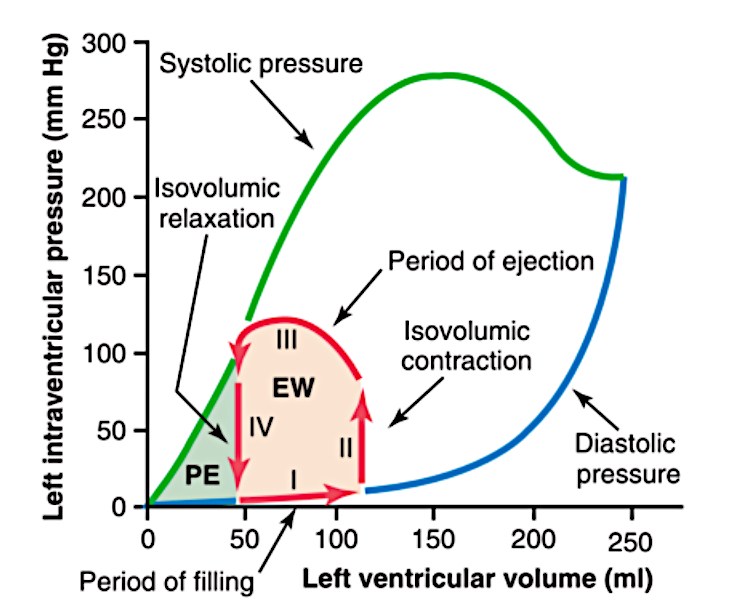
\includegraphics[width=0.5\textwidth]{images/chapt_2/pv_1.jpg}\label{fig:pv_1}}
  \subfloat[]
  {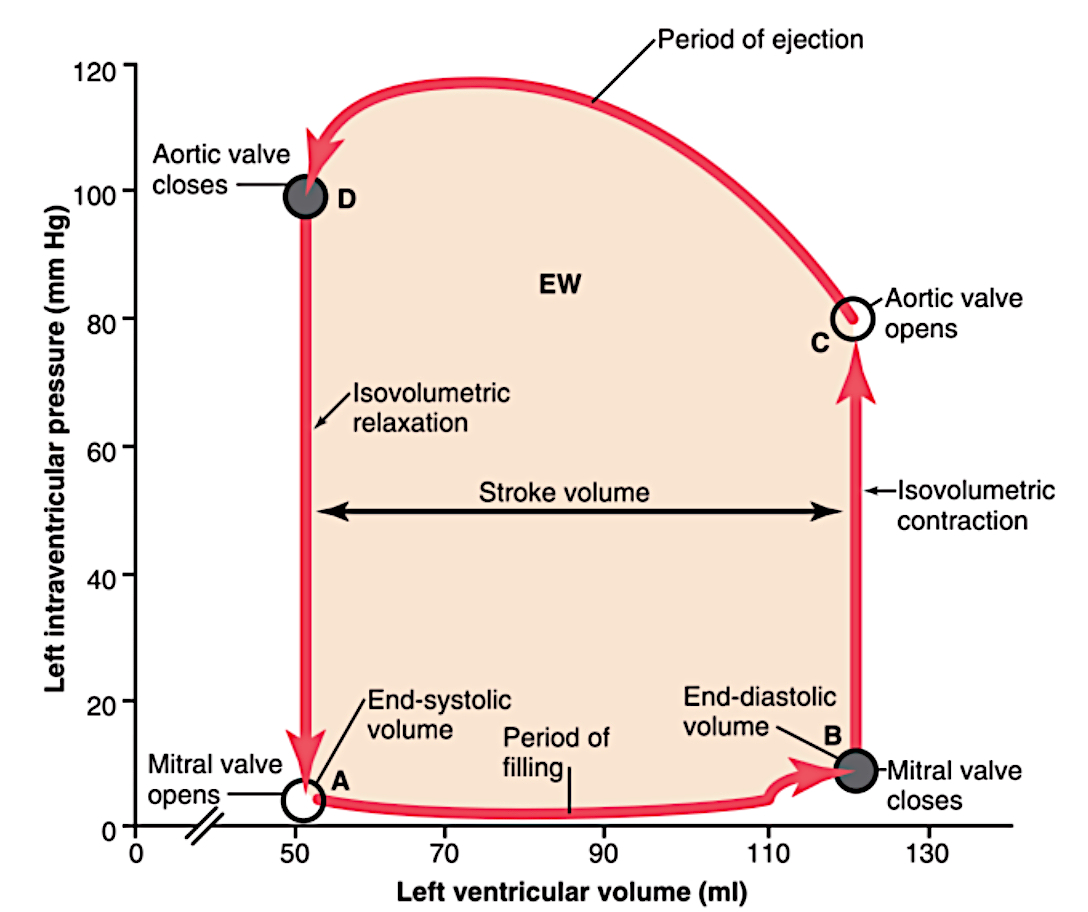
\includegraphics[width=0.5\textwidth]{images/chapt_2/pv_2_.jpg}\label{fig:pv_2}}
  \caption[P-V diagram \cite{GH20}]{(a) Working diagram of the left ventricle with the P-V diagram. (b) Close-up P-V diagram. \cite{GH20}}
  \label{fig:pv}
\end{figure}
The figure displays two curves named \textit{diastolic pressure} and \textit{systolic pressure}. Diastolic pressure is defined as the lowest point of each pulse during the relaxed state of the heart, whilst systolic pressure represents the highest point of each pulse, occurring while the heart is contracting and ejecting blood. \cite{HKS4}
The blue curve in \figurename~\ref{fig:pv_1}, representing the diastolic pressure, is determined by gradually filling the heart with higher blood volumes and subsequently measuring the diastolic pressure just before ventricular contraction occurs. It describes the heart's mechanical properties when the myocardium is in a relaxed state. The green curve in \figurename~\ref{fig:pv_1}, named systolic pressure, is plotted by measuring the systolic pressure over varying filling volumes for constant ventricle volumes. The red lines in \figurename~\ref{fig:pv_1} and \figurename~\ref{fig:pv_2} indicate the cardiac cycle and its four action phases, as described above. The line between points A and B in \figurename~\ref{fig:pv_2} depicts the period of rapid filling. The isovolumic contraction is represented by line II in \figurename~\ref{fig:pv_1}, respectively between points B and C in \figurename~ \ref{fig:pv_2}. The ejection phase is depicted by III in \figurename~\ref{fig:pv_1} and the line referred to as IV represents the period of isovolumic relaxation. The area of the work diagram, marked with EW in \figurename~\ref{fig:pv} is a measure of the work done by the heart. The P-V diagram furthermore enables calculation of the ejection fraction (EF), which describes the percentage value of the ventricle volume ejected during systole. It is determined by
\begin{equation}
  EF = \frac{SV}{EDV}*100.
 \label{eq:EF}
\end{equation}
For a healthy heart at rest, with a stroke volume of about $70 \, ml$ and an EDV of about $110-120 \, ml$, the EF amounts to about $50-60\, \%$. In cases of heart failure, the EF can decrease to about $20-25 \, \%$. Therefore, knowledge of the P-V diagram is an important prerequisite in understanding myocardial diseases. \cite{HKS4}

\section{Heart failure}
The World Health Organization (WHO) lists cardiovascular diseases (CVDs) as the global number one cause of death. In 2016, about 17.9 million people died from CVDs, representing $31 \,\%$ of all global death that year. \cite{WHO}
\\In case of heart failure, the heart is unable to provide the required amount of blood flow to the cardiovascular system in order to supply all organs and tissue with oxygen.
Heart failure does not directly represent a disease but rather a clinical syndrome. Nevertheless, the symptoms of different forms of heart failure are very similar and eventually manifest themselves in a decreased cardiac output. One acute consequence of heart failure, for example, is the perceiving shortness of breath. In the long term, however, severe heart failure can also lead to muscle weakness and a lack of concentration.
\\According to Schmidt et al. \cite{HKS4}, heart failure can be attributed to either systolic or diastolic dysfunction. Systolic dysfunction can manifest itself in several ways. One is a reduced contractility and stroke volume of the heart. Causes may be, for example, a coronary artery disease that limits oxygen supply or a preceding myocardial infarction. Secondly, there may be increased pumping resistance due to an outflow obstruction.  This may be the result of arterial hypertension, among other things. Furthermore, cardiac arrhythmias or a heart attack can lead to systolic dysfunction. \figurename~\ref{fig:sys_dys} displays the variation of the P-V diagram, comparing a normal functioning heart (dotted line) to one impaired by heart failure with a systolic dysfunction (solid line). In diastolic functional impairment, the dysfunction is evident in the course of the filling phase. This can be triggered, among other things, by reduced compliance of the myocardium due to hypertrophy or fibrosis. The change in the P-V diagram for diastolic heart failure is illustrated in \figurename~\ref{fig:dias_dys}.
\begin{figure}[ht]
  \centering
  \subfloat[]
  {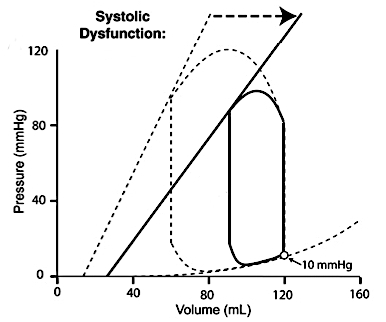
\includegraphics[width=0.5\textwidth]{images/chapt_2/sys_dys.jpg}\label{fig:sys_dys}}
  \subfloat[]
  {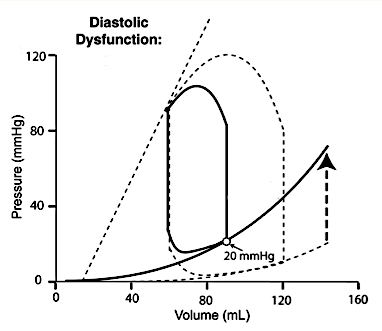
\includegraphics[width=0.5\textwidth]{images/chapt_2/dias_dys.jpg}\label{fig:dias_dys}}
  \caption[P-V diagram for heart failure]{P-V diagram for heart failure in case of (a) a systolic dysfunction and (b) a diastolic dysfunction according to \cite{HKS_pv}. The dotted lines symbolize normal heart function in comparison to the dysfunction represented by solid lines.}
  \label{fig:hf_dys}
\end{figure}
For treatment of heart failure, drug therapy using beta-blockers is initially targeted in most cases. However, if this is not successful, the use of ventricular assist devices can be a useful alternative in order to relieve the heart and provide sufficient blood flow. \cite{HKS4}

\section{Ventricular Assist Devices}
Despite heart transplantation (HTx) still being the gold standard for treatment of patients with terminal heart failure \cite{VAD2}, ventricular assist devices (VADs), as a kind of mechanical circulatory support (MCS) technology, are becoming increasingly important in treating patients with CVDs. There are two reasons for this. On the one hand, CVDs are gaining in importance due to demographic change. On the other hand, there is an increasing shortage of donor organs. \cite{VAD7}

\subsection{Therapeutic objective}
Traditionally, the therapeutic goals of VAD treatment can be divided into three categories: \textit{bridging to transplantation} (BTT), \textit{bridging to recovery} (BTR) and \textit{destination therapy} (DT). However in some cases, the classification into \textit{bridging to decision} (BTD) and \textit{bridging to transplantability} are mentioned additionally. The decision for one of these goals is based on the type of CVD and the condition the patient is in when receiving VAD assistance. \cite{VAD6}
\\In clinical practice, different classification techniques connecting the patient's condition with the estimated survival time and the need for VAD assistance are used. An overview of the relation between the Interagency Registry for Mechanically Assisted Circulatory Support (INTERMACS) Score, the New York Heart Association(NYHA)-classification and the patient's condition is presented in \tablename~ \ref{tab:Table1}.
\begin{table}[ht]
  \begin{tabularx}{\textwidth}{l|c|l|l}
    \toprule
    INTERMACS & NYHA & Patient condition & Survival time  \\
    Score & & &\\
    \midrule
    1 & IV & critical cardiogenic shock & hours \\
    2 & IV & increasing catecholamine demand & days \\
    3 & IV & stable under inotropics & a week \\
    4 & IV & frequent decompensation & weeks-month \\
    5 & IV & rest discomfort/ not resilient & weeks-month \\
    6 & IV & rest discomfort/ merely resilient & month \\
    7 & IIIb & merely resilient & one year survival rate: \\
     & & & 50-70\% \\
     \bottomrule
  \end{tabularx}
  \caption[Relation between INTERMACS Score and NYHA-classification]{Relation between INTERMACS Score, NYHA-classification, patient condition and approximate survival time based on \cite{VAD5}.}
  \label{tab:Table1}
\end{table}
The INTERMACS Score, which is based on data from patients which have received VAD treatment, links the need for a VAD and the appropriate time frame in which the device needs to be implanted. It is of high importance in deciding the therapeutic objective for VAD treatment. \cite{VAD7}
\\The goal of \textit{bridging to transplantation} is of great relevance with patients in NYHA-IV stadium showing hemodynamical instability. Due to a heart transplantation being the desired final treatment for these patients, there must be no contraindication to HTx. In case the patient does show a contraindication such as malignant tumors or an uncontrollable sepsis, the therapeutic objective changes from BTT to DT. In order for a treatment with a VAD as destination therapy being indicated, all conservative treatment options need to be exhausted. Due to the ever-growing shortage of donor organs, DT as a therapeutic approach in patients with heart insufficiency will become more relevant in the future even in cases usually suited for heart transplantation. \cite{VAD7} There may occur some cases first contraindicating HTx, for which the concentration later on may dissolve. These indicate a therapy based on a \textit{bridging to transplantability} goal. \cite{VAD6}
\\The indication for a \textit{bridging to recovery} approach is twofold. Either the patient shows heart failure as a result of ischemia reperfusion damage or due to infectious genesis. In the first case the myocardium usually is able to recover within a few days, whereas in the second one the potential and the time necessary for recovery depend on how badly the tissue is damaged. In either scenario, a weaning from the VAD is an essential part of therapy. \cite{VAD7}
\\If a patient is admitted in cardiogenic shock and medical treatment is not sufficient, \textit{bridging to decision} becomes a relevant form of therapy. By providing the patient with a VAD, a more accurate assessment of the patient's condition is possible.
Based on this, the decision on further treatment can be analysed more thoroughly. \cite{VAD6}

\subsection{Technology}
Since the first artificial blood-pump has been implanted in 1963, technology of VADs has improved significantly \cite{VAD9}.
\\The general aim of ventricular assist devices is to provide mechanical support in pumping blood through the human body with the heart remaining inside the patient's body. Despite there being several types of VADs, all of them are working according to the same principle. Blood is taken from the circulatory system through the pump's inlet and ejected at another location via the pump's outlet. \cite{VAD1}
\\VADs are differentiated by three criteria: localization of the device inside the human body, flow profile and implantation strategy.
\\Regarding localization of the assistance device, three different options exist. With around $93\, \%$ of all implemented devices, the most commonly used ones are left ventricular assist devices (LVADs). \cite{VAD7} LVADs are connected to the left ventricle, from where they are pumping blood into the aorta \cite{VAD4}. The second localization option is placing the device as support for the right ventricle. These devices are therefore called right ventricular assist devices (RVADs). RVADs are positioned in a way that blood is taken from the right atrium and ejected into the pulmonary artery. \cite{VAD7} In some cases, RVADs in combination with the aforementioned LVADs are used to build a biventricular assist device (BVAD). This type of heart support is mainly used for more severe heart diseases with a high risk of developing right heart failure. \cite{VAD11}
\\The flow profile, as the second criterion for VAD distinction, is represented by pulsatile and continuous flow devices. Assistance with pulsatile devices can either be implemented to support the heart in a counter pulsation approach, working synchronous to the heart cycle, or as an asynchronous support. The most commonly known type of pulsatile device is a pneumatically driven pump ventricle. \cite{VAD1}
However, according to the INTERMACS, over $95\, \%$ of all implanted devices are continuous flow devices \cite{VAD8}. These, in their most commonly used form, are electrically driven rotational blood pumps. A technological difficulty with these devices is the high probability of blood damage due to small gaps and very high rotational speed. However, these devices enable a dynamic adaption to the patient's physiological needs by being able to quickly adjust parameters such as the motor current. The possibility to keep track of these signal characteristics furthermore makes it possible to detect malfunctions or misplacement of the pump. \cite{VAD1}
\\Implantation of the VADs can be performed in one of three ways: paracorporeal, intracorporeal or percutaneous \cite{VAD7}. For VAD systems which follow a paracorporeal approach, only the in- and outflow cannulas are located inside the human body. The cannulas are connecting the pump located outside the body with the ventricle and the vessels. Due to the pump being placed outside of the patient's body, these systems provide the option for pediatric MCS. This is not possible for most other systems due to the device being too large to fit inside a child's body. \cite{VAD10} One example for paracorporeal systems are the aforementioned pneumatically driven pump ventricles \cite{VAD1}. In contrast to the paracorporeal devices, where the pump itself as well as its control unit are situated outside the body, in percutaneous devices the pump is placed inside the body. The control unit, however, remains outside the patient's body and is connected to the pump via leads. The intracorporeal devices are fully implanted into the body. \cite{VAD10}
\\As far as the other two criteria for VAD differentiation are concerned, all combinations of localization and flow control are possible \cite{VAD10}. As an example of a percutaneous device, \cite{VAD7} names the Impella 2.5, a rotary blood pump with continuous flow used for left ventricular assistance.
\\The proportions of different VAD types and therapeutic goals, as based on the International Mechanically Assisted Circulatory Support (IMACS) register are illustrated in \tablename~ \ref{tab:Table2}.
\begin{table}[ht]
  \centering
  \begin{tabular}{cc|cc}
    \toprule
    \multicolumn{2}{c|}{VAD type} &
    \multicolumn{2}{c}{Therapeutic objective} \\
    \midrule
    LVAD & 93\% & DT & 40\%\\
    BVAD & 4\% & BTD & 30\%\\
    TAH & 2\% & BTT & 29\%\\
    unknown & 0.1\% & others (BTR, ...) & 1\%\\
    RVAD & 0.05\% & &\\
    \bottomrule
\end{tabular}
  \caption[Distribution of VAD types and therapeutic objectives]{Percentages of VAD types and therapeutic objectives in mechanical heart support based on \cite{VAD7}.}
  \label{tab:Table2}
\end{table}
